\chapter{Setup}
To do the task laid out, the following equipment was used:

\begin{itemize}
\item 6 Degrees of Freedom Universal Robot
\item Logitech Webcam 1080p
\item MATLAB
\item \lego Duplo bricks
\item Parallel Gripper
\end{itemize}

The robot cell is shown in \autoref{fig:workarea}. The red square marks the zone where the bricks are placed. The Universal Robot (UR) can then grab them with a parallel gripper. The green zone marks the drop off zone. Here the UR delivers the assembled figure.

\begin{figure}[h]
\centering
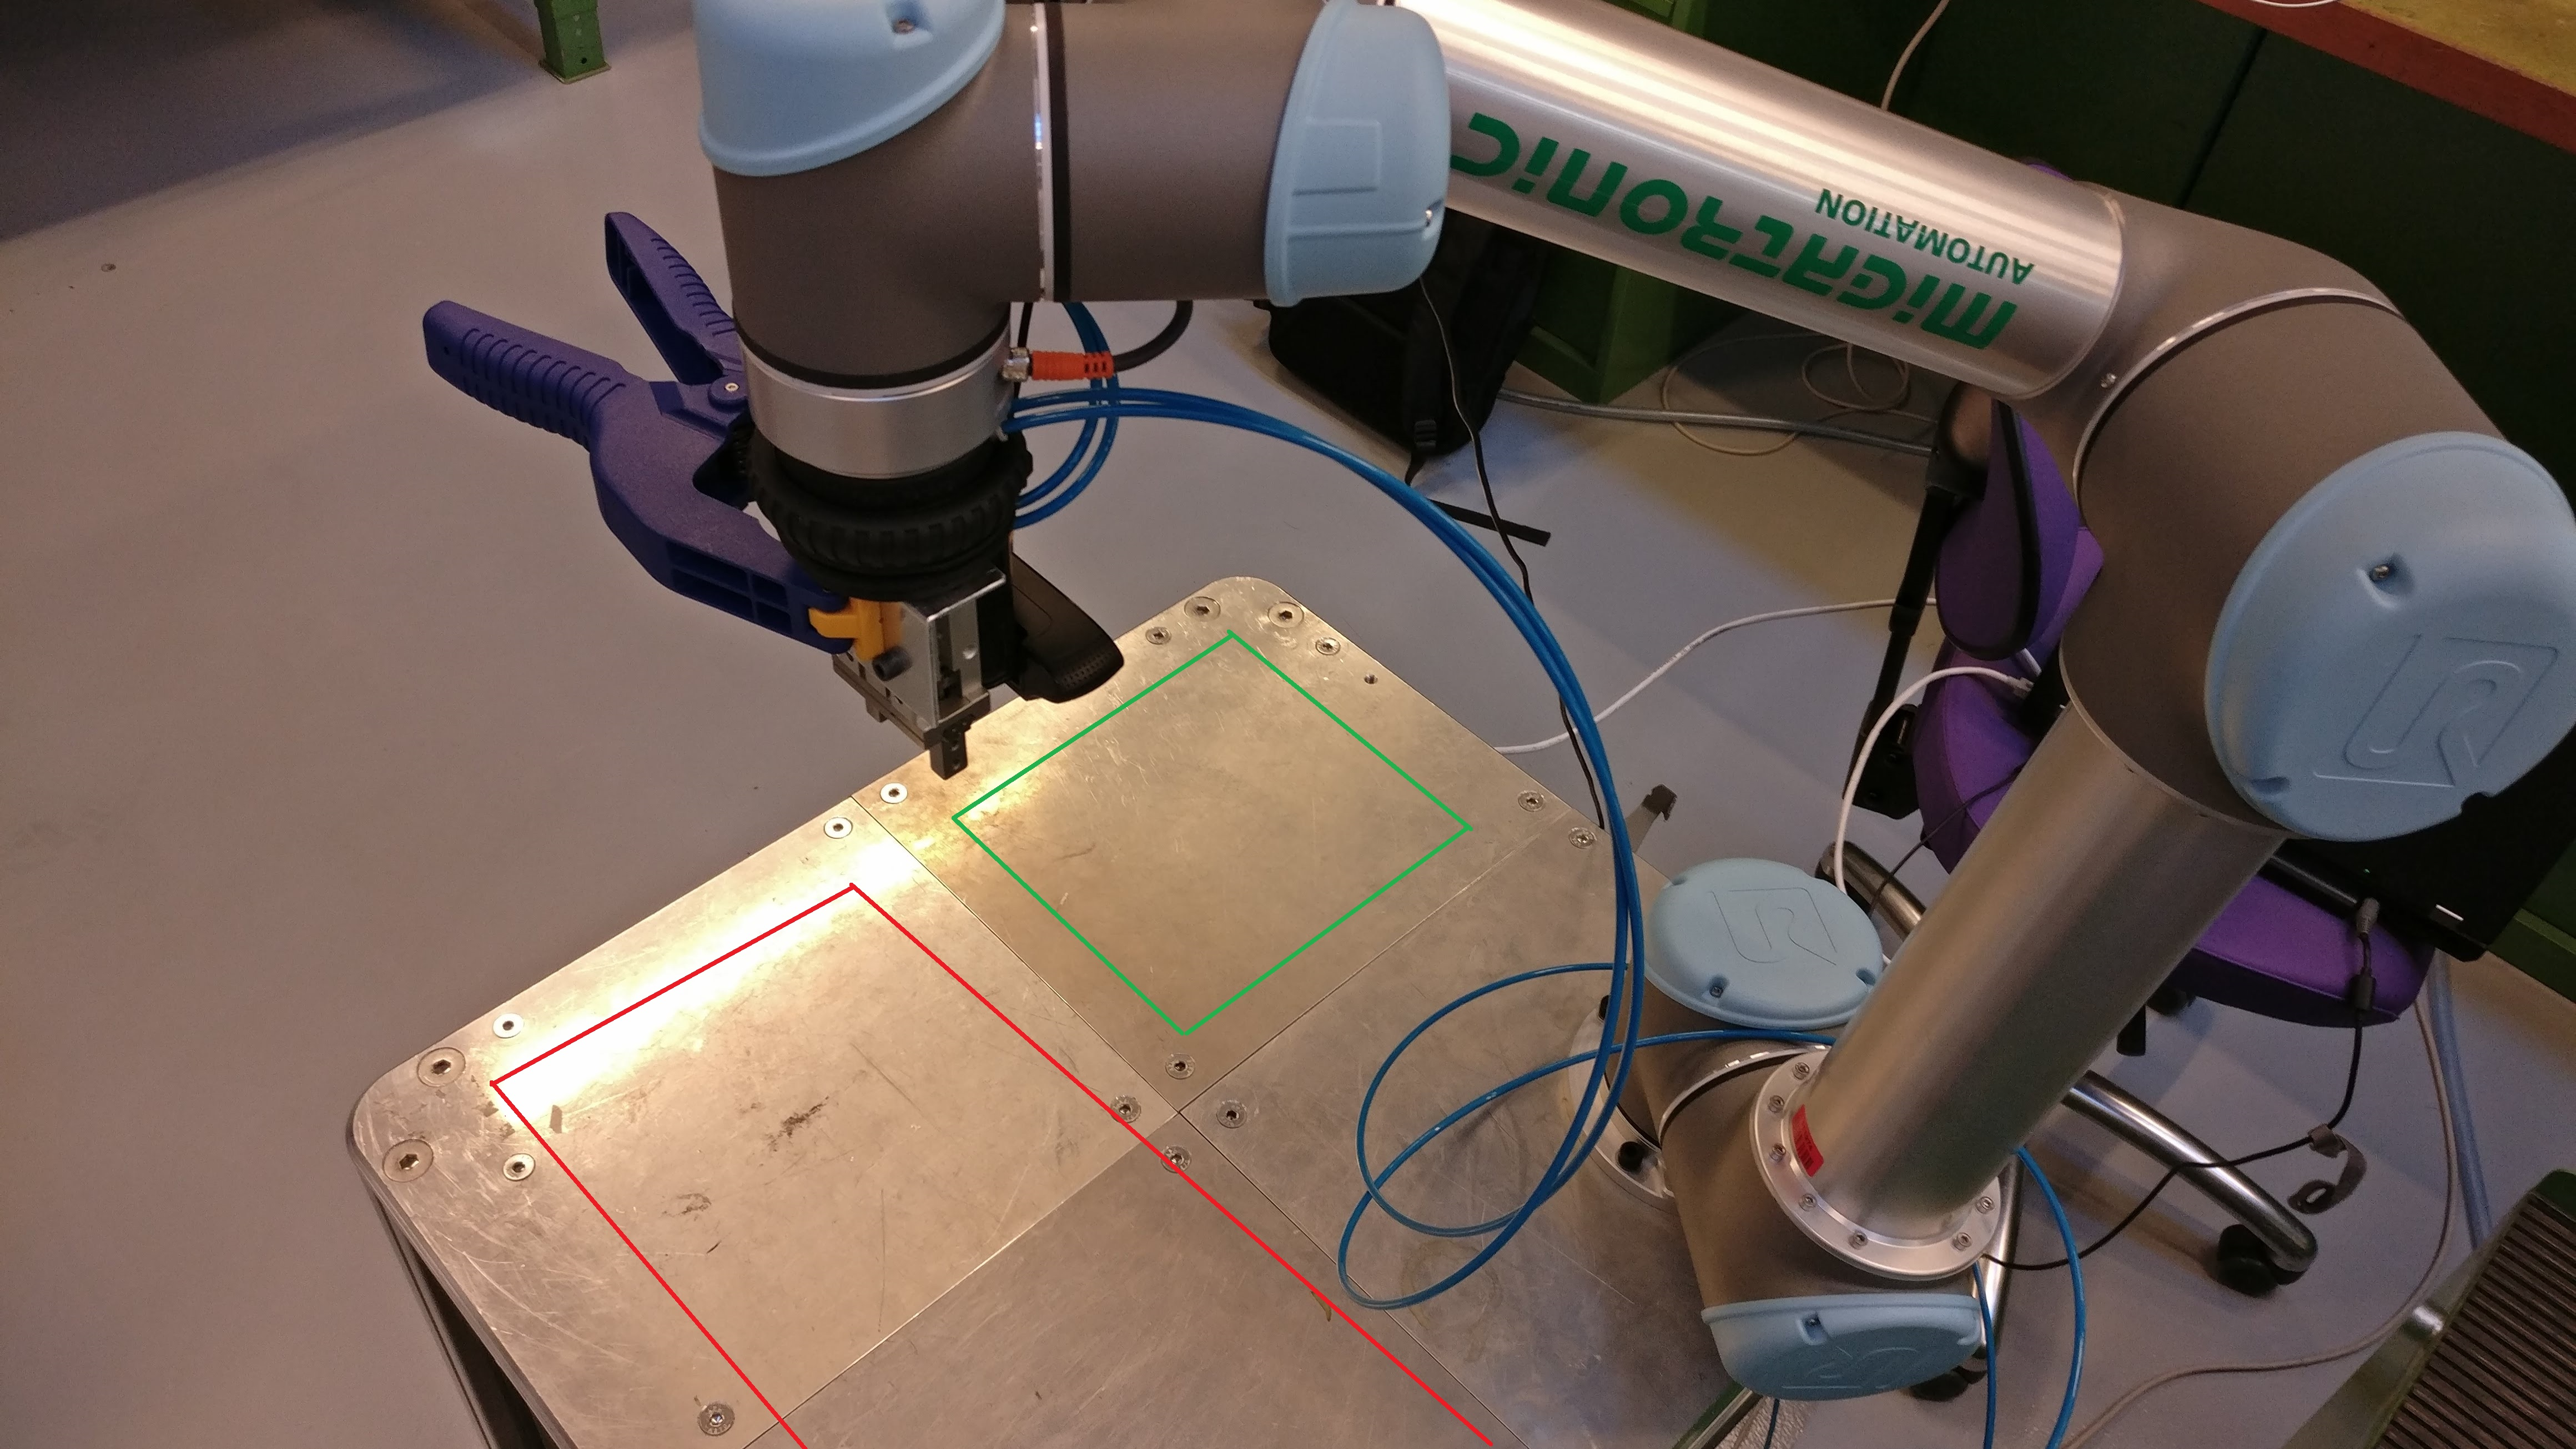
\includegraphics[width=\textwidth]{figures/workarea.jpg}
\caption{}
\label{fig:workarea}
\end{figure}

The camera was mounted to the tool, \autoref{fig:tool_cam}, as there were no other places to mount it. The benefits of this approach are that the camera does not obstruct the robot when it is moving and that the cameras frame is known when the tool is known, except it is flipped on one of the axes.

\begin{figure}[h]
\centering
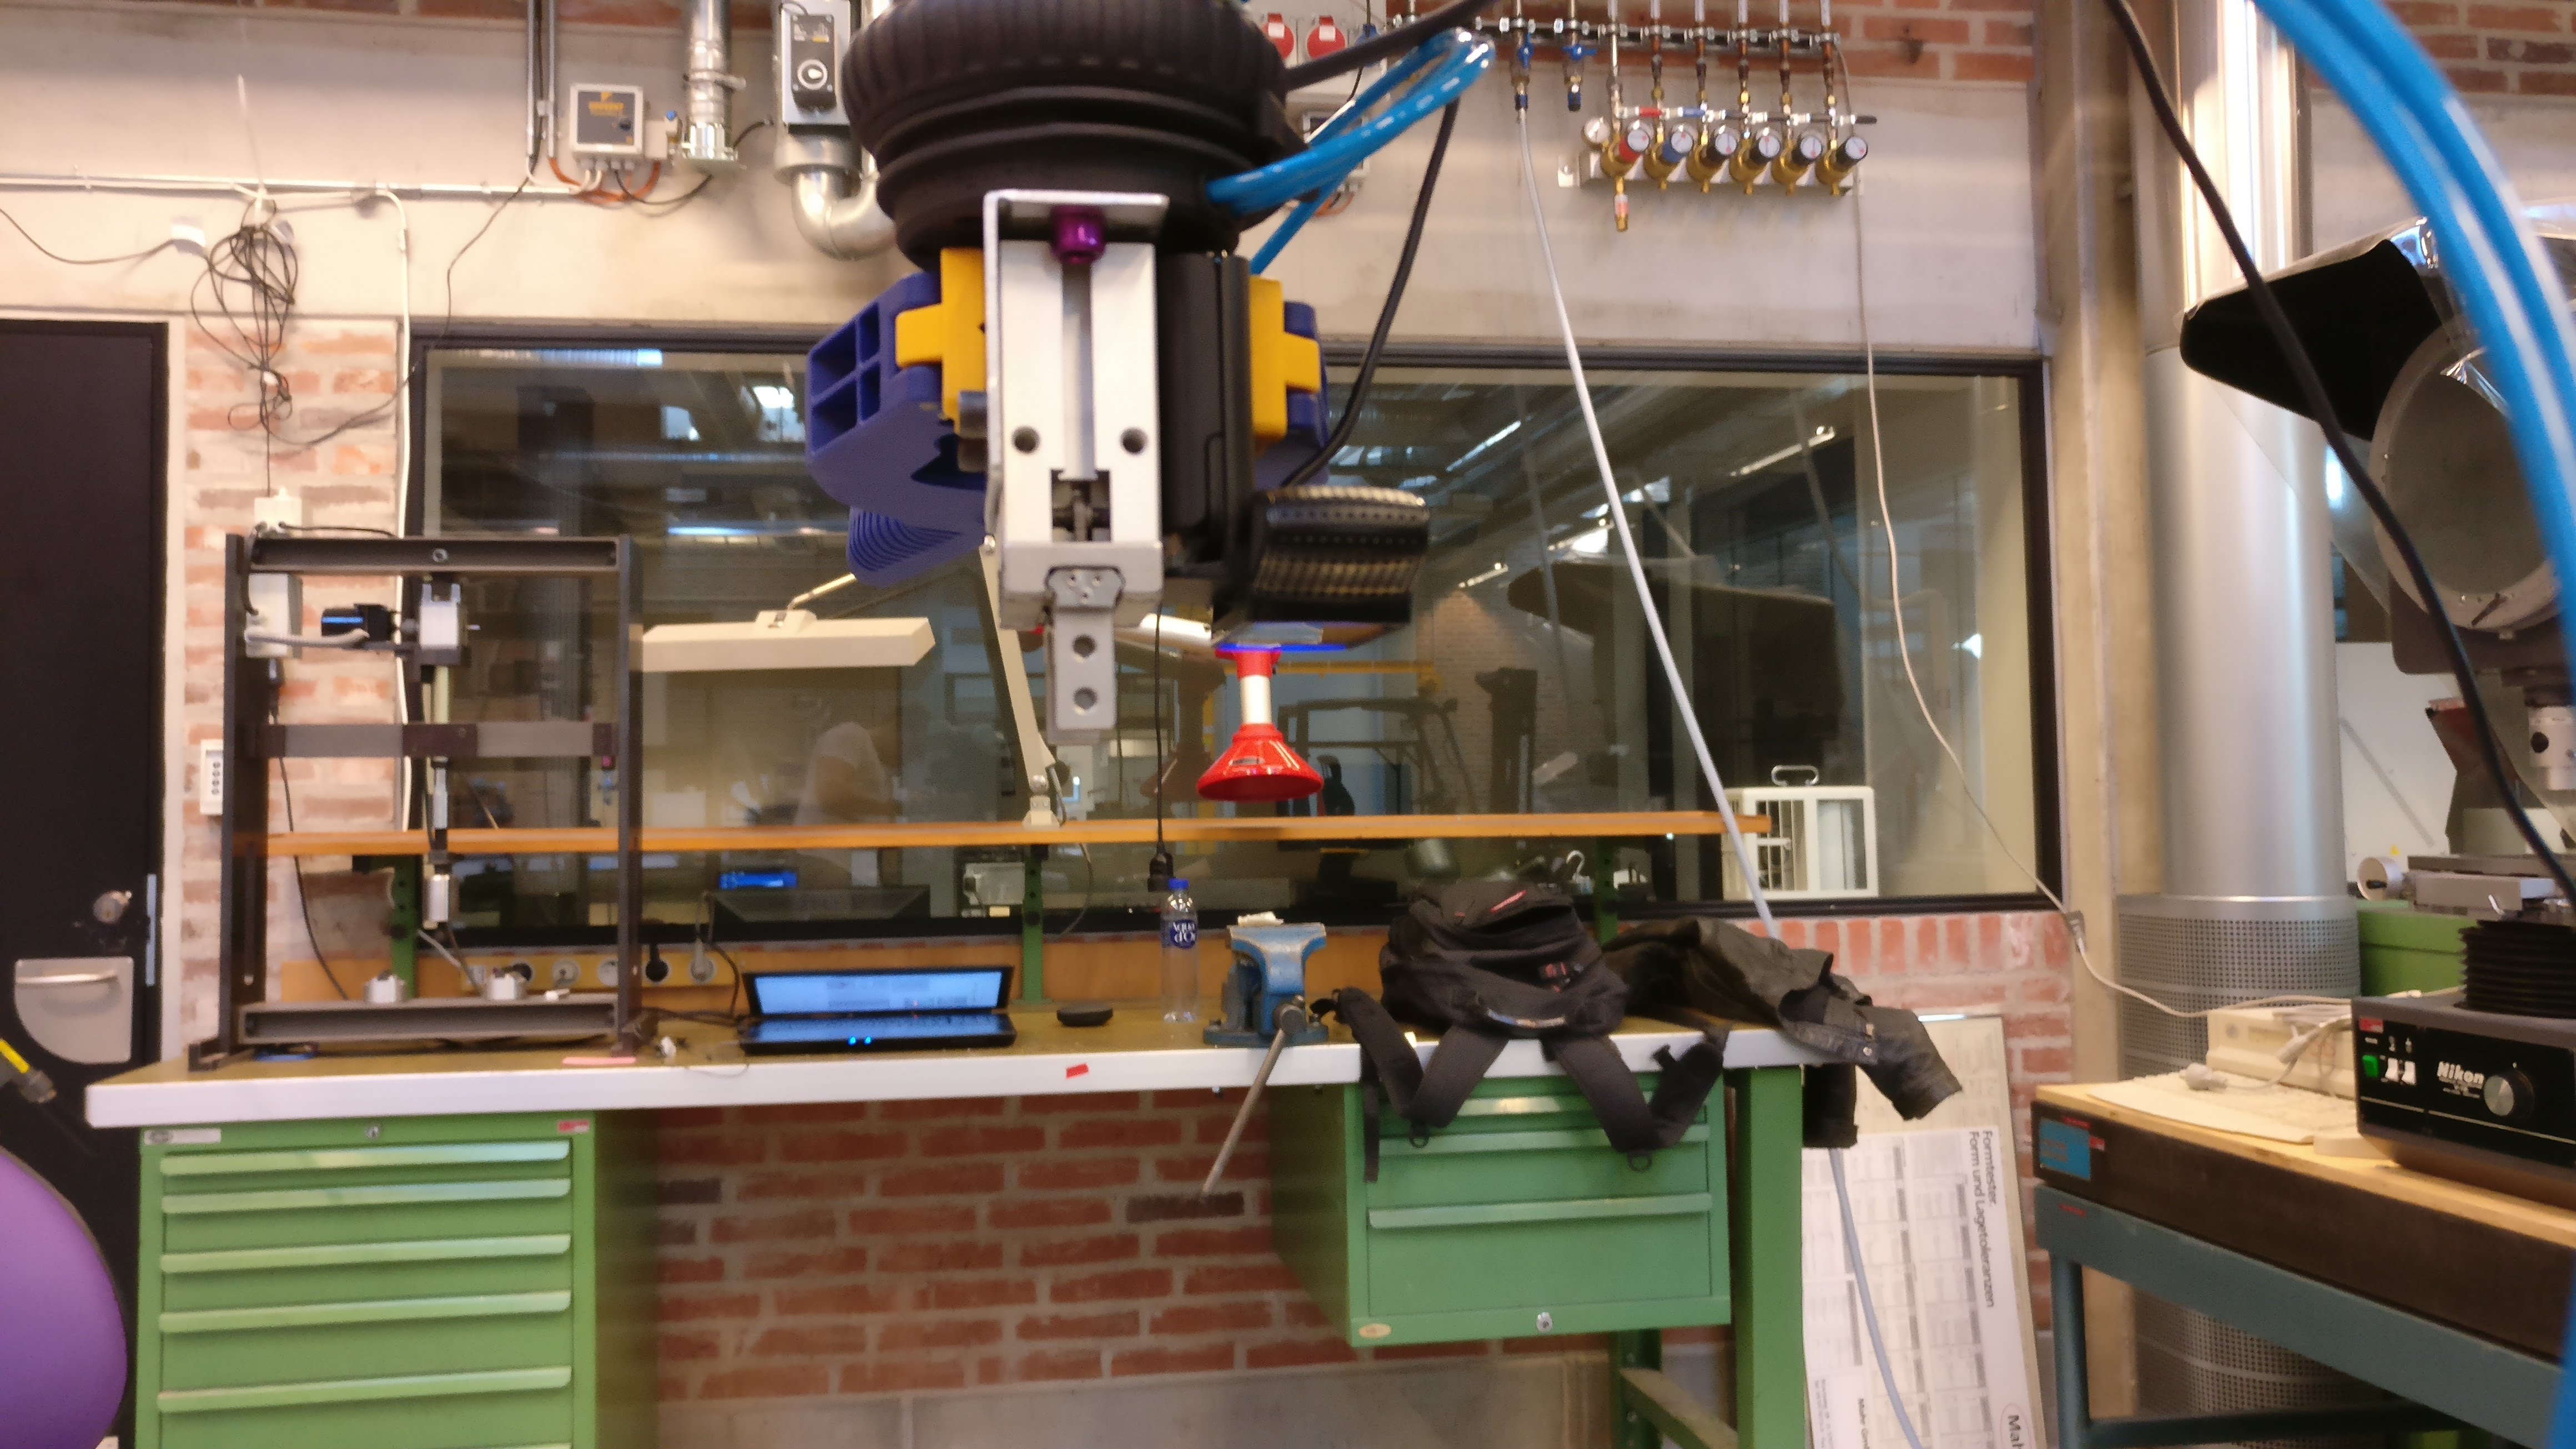
\includegraphics[width=0.7\textwidth]{figures/tool_cam.jpg}
\caption{}
\label{fig:tool_cam}
\end{figure}